\newcommand{\CLASSINPUTinnersidemargin}{18mm}
\newcommand{\CLASSINPUToutersidemargin}{12mm}
\newcommand{\CLASSINPUTtoptextmargin}{20mm}
\newcommand{\CLASSINPUTbottomtextmargin}{25mm}

\documentclass[10pt,conference,a4paper]{IEEEtran}%

% Using "no-tilde" option with babel package solves a compilation
% error when using more than 100 characters on float's captions.
\usepackage[english]{babel}
%\usepackage[spanish,es-nosectiondot,es-tabla,es-nolists]{babel}
% Requiere spanish.ldf para babel versión >= 5.0 (feb 2007) Versiones anteriores
% interfieren con IEEEtran, especialmente en el formato de los títulos de
% section y subsection, por lo que se recomienda no utilizarlas. Si aun así
% se utilizan, comentar la lí­nea anterior y descomentar la siguiente
%\usepackage[spanish]{babel}

% Intenta corregir los efectos indeseados de babel
\renewcommand{\thesubsection}{\Alph{subsection}}
\renewcommand{\thesubsubsection}{\arabic{subsubsection}}
\addto\extrasspanish{\def\tablename{Tabla}}
\addto\extrasspanish{\def\figurename{Fig.}}

% For english version, comment or delete all the lines above up to documentclass

\usepackage[utf8x]{inputenc}
% For codification latin1 (ISO 8859-1) instead of UTF-8.
% Comment the line above and uncomment the line below:
%\usepackage[latin1]{inputenc}

\usepackage{amsmath,amsfonts,amssymb}
\usepackage{times}
\usepackage{graphicx}
\usepackage{url}
% Prevents floats from appearing in secctions in which they werent declared
%\usepackage[above,below]{placeins}

% Other usefull Packages
%\usepackage[caption=false]{subfig}  % Subfigures (parametter required).
%\usepackage{colortbl}        % Colored tables.
%\usepackage{multirow}        % Vertical joined cell tables.
%\usepackage{cite}          % Compact refference lists.
%\usepackage{pstool}          % Generates .ps or .pdf from psfrag

\DeclareGraphicsExtensions{.png,.eps,.ps,.pdf,.jpg}

% Hack para corregir las cabeceras de tablas de IEEEtran. Con esto figuras y tablas
% tienen el mismo formato.
\makeatletter \def\@IEEEtablestring{} \makeatother


% --------------------------------------------------------------------------------
% Content Starts Here
% --------------------------------------------------------------------------------

\title{China Case}

\author{%
\IEEEauthorblockN{Zamora, Sa\'ul}
\IEEEauthorblockA{aleks279@gmail.com}
\IEEEauthorblockA{200835773}

\IEEEauthorblockN{Rojas, Allan}
\IEEEauthorblockA{aallanrd@gmail.com}
\IEEEauthorblockA{200941386}
}


\begin{document}

\maketitle

% The abstract, sections and subsections don't need to be closed.
\begin{abstract}
  Even when most of us take it for granted, Internet access is not as common as one would believe. For 60 percent of the world's population, internet access is as common as flying cars; either because they live in a remote area or due to censorship on part of the local goverment.
  The Outernet project hopes to succeed in these cases by getting a new breed of satellite-based communication off the ground and promising to give even the most remote corners of the globe access to the whole of humanity's collective knowledge.
\end{abstract}

\section{The Outernet Project}
The Outernet is the brainchild of the same-named New York based tech company. It's a free content distribution system that would provide basic web access broadcast via a series of geostationary and LEO satellites, as well as cube satellites using a combination of datacasting and user datagram protocols.
Datacasting is exactly what it sounds like: the wide area broadcast of data using radio waves rather than physical mediums (like cable, telephone, or powerlines). User Datagram Protocols, or UDP, is very similar to conventional over-the-air radio or television broadcasts in that it's uni-directional. The data is beamed from its source to any device within range and there's no guarantee that it will be received, just like radio stations broadcast their signals without regard to which or how many radios are currently in range to catch it.
UDP is one of the most basic forms of Internet protocol. Invented back in 1980, it's a connectionless transmission model—in that it doesn't require someone to be on the other end of the line when the data is sent.

\subsection{Radio for the digital age}
The Outernet would behave as a modern analog to conventional radio broadcast. The signal would originate from a single location and travel accross a variety of wavelengths until it hits a suitable receiver where the end user can flip between "stations" by modulating the received frequency.
Rather than relying on terrestrial radio stations, the Outernet bounces its signal up to a series of satellites then back down to a suitable receiver. This receiver doubles as a Wi-Fi hotspot then connects to a computer or mobile device and transfers the received data as a digital file. And since there is no two-way communication the system requires much lower bandwidth and, therefore, much less money to operate.

\subsection{Humanity's public library}
On the information side, the company has begun forming what it calls a "core archive" of knowledge based on information gleaned from 5,000 Wikipedia entries, Project Gutenberg, and a smattering of copyright-free e-books. The early plan—which definitely has some kinks to work out—is to crowdsource what content is broadcast and make decisions based on user requests and upvotes.
What's more, since the system in uni-directional, it's far more difficult to censor—just as shortwave radios served as vital information lifelines for those stuck behind the Iron Curtain during the Cold War. Initially funded by a news media investment company, Outernet's mission is to provide free, anonymous, educational information, available to regions facing government censorship or otherwise off the grid.
In August this year, the startup started beaming this data across 200MB of leased geostationary satellite bandwidth, which reaches throughout North America and most of Western Europe, with plans to expand to the rest of the globe by July, 2015. Should the company's IndieGoGo fundraising efforts work out, it could boost the daily broadcast limit to 100GB in the near future.
A single receiver in a central African village, according to Karim's recent Ted Talk, could provide reams of valuable information to as many as 300 local residents—everything from agricultural texts to health, and human services. "If you were in the vicinity of a hotspot receiving the data from the satellite, you would be able to connect with Outernet on your phone and see Librarian—our index software—as if it was just an offline website," he said. "There you would find the data, stored in files."
In addition to disseminating evergreen information, the Outernet could very well also be used for emergency alert broadcasts which would be updated multiple times an hour instead of the average rate of once every week or so.

\subsection{An Ambitious Project}
Some internet is way better than no internet. And with estimates placing global internet reach on par with what Outernet can provide still 15 to 20 years away, the Outernet could provide a valuable stop-gap service until conventional 'net access becomes viable.
To that end, Outernet has partnered with the World Bank in South Sudan to perform a test run of the service next July. Should it prove successful, the company hopes to increase its coverage area and begin offering the self-contained receivers, called "lanterns," from its Indiegogo campaign around that time.
And even if the Outernet itself fails to take off, it is far from the only free access system currently in development. Two of the biggest names in tech have already thrown their weight behind similar strategies. Google's Project Loon would see fleets of high altitude balloons bouncing 3G signals from the straosphere back down to the Earth's most remote regions. Facebook's Internet.org, on the other hand, envisions swarms of drones and LEO satellites performing the same function. Even SpaceX is rumored to be building a satellite fleet to bring internet to the far-flung corners of the globe.

\section{China's Great Firewall}
The Great Firewall of China (GFW) is the combination of legislative actions and technologies enforced by the People's Republic of China to regulate the Internet domestically. Its role in the Internet censorship in China is to block access to selected foreign websites and to slow down cross-border internet traffic. The effect includes: limiting access to foreign information sources, blocking foreign internet tools (e.g. Google search, Facebook, Twitter etc.) and mobile apps, and requiring foreign companies to adapt to domestic regulations. Besides censorship, the GFW has also influenced the development of China's internal internet economy by nurturing domestic companies and reducing the effectiveness of products from foreign internet companies.
China's special administrative regions such as Hong Kong and Macau are not affected by the project, as SARs have their own governmental and legal systems and therefore enjoy a high degree of autonomy. Nevertheless, it was reported that the central government authorities have been closely monitoring the Internet use in these regions.

\subsection{History}
The political and ideological background of the GFW Project is considered to be one of Deng Xiaoping’s favorite sayings in the early 1980s: "If you open the window for fresh air, some flies will be blown in". The saying is related to a period of the economic reform of China that became known as the "socialist market economy". Superseding the political ideologies of the Cultural Revolution, the reform led China towards a market economy and opened up the market for foreign investors. Nonetheless, despite the economic freedom, values and political ideas of the Communist Party of China have had to be protected by "swatting flies" of other unwanted ideologies.
The Internet in China arrived in 1994, as the inevitable consequence of and supporting tool for the "socialist market economy". Gradually, while Internet availability has been increasing, the Internet has become a common communication platform and tool for trading information.
The Ministry of Public Security took initial steps to control Internet use in 1997, when it issued comprehensive regulations governing its use. The key sections, Articles 4–6, are:
\emph{Individuals are prohibited from using the Internet to: harm national security; disclose state secrets; or injure the interests of the state or society. Users are prohibited from using the Internet to create, replicate, retrieve, or transmit information that incites resistance to the PRC Constitution, laws, or administrative regulations; promoting the overthrow of the government or socialist system; undermining national unification; distorting the truth, spreading rumors, or destroying social order; or providing sexually suggestive material or encouraging gambling, violence, or murder. Users are prohibited from engaging in activities that harm the security of computer information networks and from using networks or changing network resources without prior approval.}
In 1998, the Communist Party of China feared that the China Democracy Party (\emph{CDP}) would breed a powerful new network that the party elites might not be able to control. The CDP was immediately banned, followed by arrests and imprisonment. That same year, the GFW project was started. The first part of the project lasted eight years and was completed in 2006. The second part began in 2006 and ended in 2008.

\subsection{Blocking Methods}
The system blocks content by preventing IP addresses from being routed through. It consists of standard firewalls and proxy servers at the Internet gateways. The system also selectively engages in DNS poisoning when particular sites are requested. The government does not appear to be systematically examining Internet content, as this seems to be technically impractical.
Researchers at the University of California, Davis, and at the University of New Mexico said that the censorship system is not a true firewall since banned material is sometimes able to pass through several routers or through the entire system without being blocked.
Some commonly used technical methods for censoring are:

\begin{itemize}
  \item IP Blocking
  \item DNS spoofing, filtering and redirection
  \item URL filtering
  \item Packet filtering
  \item Man-in-the-middle attack
  \item TCP connection reset
  \item VPN blocking
  \item Network enumeration
\end{itemize}

\section{Protests in China}
Despite strict government regulations, the Chinese people are continuing to protest against their government’s attempt to censor the Internet. The more covert protesters will set up secure SSH and VPN connections using tools such as UltraSurf. They can also utilize the widely available proxies and virtual private networks to fanqiang, or bypass the GFW. Active protest is not absent. Chinese people will post their grievances online, and on some occasions, have been successful. In 2003, the death of Sun Zhigang, a young migrant worker, sparked an intense, widespread online response from the Chinese public, despite the risk of the government’s punishment. A few months later, Premier Wen Jiabao abolished the Chinese law that led to the death of Sun. Ever since, dissent has regularly created turmoil on the Internet in China. Also in January 2010, when Google announced that it will no longer censor its Web search results in China, even if this means it might have to shut down its Chinese operations altogether, many Chinese people went to the company’s Chinese offices to display their grievances and offer gifts, such as flowers, fruits and cigarettes.

\subsection{The Umbrella Revolution}
A series of sit-in street protests, often called the Umbrella Revolution, occurred in Hong Kong from 26 September to 15 December 2014. The protests began after the Standing Committee of the National People's Congress (\emph{NPCSC}) issued a decision regarding proposed reforms to the Hong Kong electoral system. The decision was widely seen to be highly restrictive, and tantamount to the Chinese Communist Party (\emph{CCP})'s pre-screening of the candidates for the leader of Hong Kong.
Students led a strike against the NPCSC's decision beginning on 22 September 2014, and the Hong Kong Federation of Students and Scholarism started protesting outside the government headquarters on 26 September 2014. On 28 September, events developed rapidly. The Occupy Central with Love and Peace movement announced the beginning of their civil disobedience campaign. Students and other members of the public demonstrated outside government headquarters, and some began to occupy several major city intersections. Protesters blocked both east–west arterial routes in northern Hong Kong Island near Admiralty. Police tactics – including the use of tear gas – and triad attacks on protesters led more citizens to join the protests and to occupy Causeway Bay and Mong Kok. The number of protesters peaked at more than 100,000 at any given time, overwhelming the police thus causing containment errors.
Government officials in Hong Kong and in Beijing denounced the occupation as "illegal" and a "violation of the rule of law", and Chinese state media and officials claimed repeatedly that the West had played an "instigating" role in the protests, and warned of "deaths and injuries and other grave consequences". The protests precipitated a rift in Hong Kong society, and galvanised youth – a previously apolitical section of society – into political activism or heightened awareness of their civil rights and responsibilities. Not only were there fist fights at occupation sites and flame wars on social media, family members found themselves on different sides of the conflict.

\subsection{Political Background}
As a result of negotiations and the 1984 agreement between China and Britain, Hong Kong was returned to China and became its first Special Administrative Region on 1 July 1997, under the principle of "one country, two systems". Hong Kong has a different political system from mainland China. Hong Kong's independent judiciary functions under the common law framework. The Hong Kong Basic Law, the constitutional document drafted by the Chinese side before the handover based on the terms enshrined in the Joint Declaration, governs its political system, and stipulates that Hong Kong shall have a high degree of autonomy in all matters except foreign relations and military defence. The declaration stipulates that the region maintain its capitalist economic system and guarantees the rights and freedoms of its people for at least 50 years after the 1997 handover. The guarantees over the territory's autonomy and the individual rights and freedoms are enshrined in the Hong Kong Basic Law, which outlines the system of governance of the Hong Kong Special Administrative Region, but which is subject to the interpretation of the Standing Committee of the National People's Congress (\emph{NPCSC}).
The leader of Hong Kong, the Chief Executive, is currently elected by a 1200-member Election Committee, though Article 45 of the Basic Law states that "the ultimate aim is the selection of the Chief Executive by universal suffrage upon nomination by a broadly representative nominating committee in accordance with democratic procedures." A 2007 decision by the Standing Committee opened the possibility of selecting the Chief Executive via universal suffrage in the 2017 Chief Executive election, and the first round of consultations to implement the needed electoral reforms ran for five months in early 2014. Chief Executive CY Leung then, per procedure, submitted a report to the Standing Committee inviting them to deliberate whether it is necessary to amend the method of selection of the Chief Executive.
As early as January 2013, legal scholar Benny Tai published an article by launching a non-violent civil disobedience of occupying Central if the government's proposal failed to satisfy the "international standards in relation to universal suffrage". A group called the Occupy Central with Love and Peace (\emph{OCLP}) was formed in March 2013 and held rounds of deliberations on the electoral reform proposals and strategies. In June 2014, the OCLP conducted a "civic referendum" on its own electoral reform proposal in which 792,808 residents, equivalent to over one fifth of the registered electorate, participated.
In June 2014, the State Council issued a white paper called The Practice of the 'One Country, Two Systems' Policy in the Hong Kong Special Administrative Region claiming "comprehensive jurisdiction" over the territory. "The high degree of autonomy of the HKSAR [Hong Kong Special Administrative Region] is not full autonomy, nor a decentralised power," it said. "It is the power to run local affairs as authorised by the central leadership."

\section{China's Connections}
An important characteristic of the Chinese internet is that online access routes are owned by the PRC government, and private enterprises and individuals can only rent bandwidth from the state. The first four major national networks, namely CSTNET, ChinaNet, CERNET and CHINAGBN, are the "backbone" of the mainland Chinese internet. Later dominant telecom providers also started to provide internet services.
In 2015 January, China added seven new access points to the world’s internet backbone, adding to the three points that connect through Beijing, Shanghai, and Guangzhou.
Public internet services are usually provided by provincial telecom companies, which sometimes are traded between networks. internet service providers without a nationwide network could not compete with their bandwidth provider, the telecom companies, and often run out of business. The interconnection between these networks is a big concern for internet users, since internet traffic via the global internet is quite slow. However, major internet services providers are reluctant to aid rivals.

\begin{figure}[htb]
	\centering
		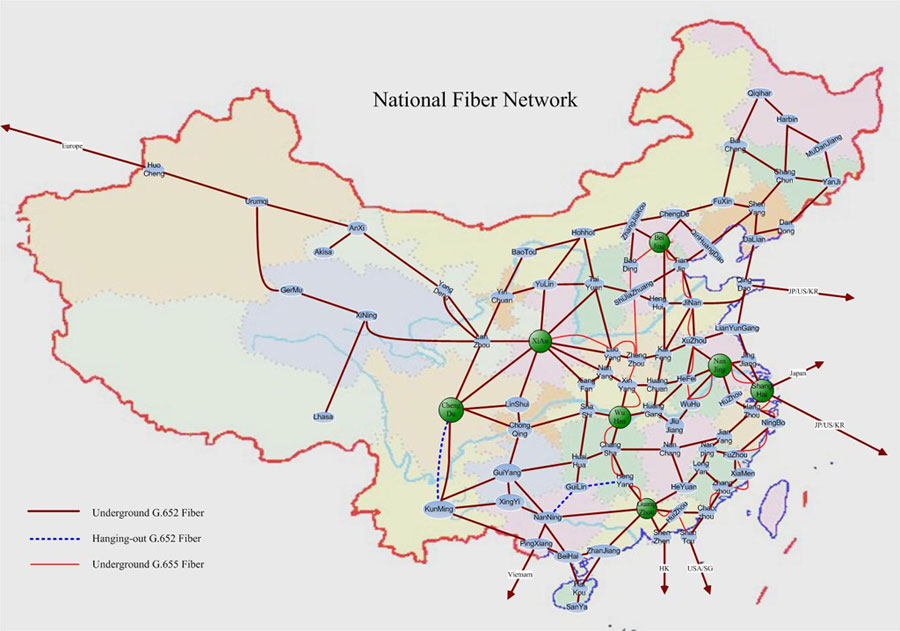
\includegraphics[width=\columnwidth]{images/map.jpg}
		\caption{China Connections Map}
	\label{fig:graph}
\end{figure}

\begin{figure}[htb]
	\centering
		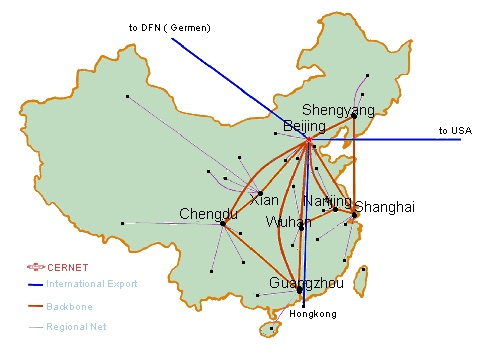
\includegraphics[width=\columnwidth]{images/cyber_map}
		\caption{China Cyber Map}
	\label{fig:graph}
\end{figure}

\begin{thebibliography}{2}
  \bibitem{anon} Gizmodo.com. (2018). [online] Available at: \texttt{https://gizmodo.com/what-is-the-outernet-and-is-it-the-future-of-the-intern-1659647614}
  \bibitem{wiki} En.wikipedia.org. (2018). Great Firewall. [online] Available at: \texttt{https://en.wikipedia.org/wiki/Great\_Firewall}
  \bibitem{wiki2} En.wikipedia.org. (2018). 2014 Hong Kong protests. [online] Available at: \texttt{https://en.wikipedia.org/wiki/2014\_Hong\_Kong\_protests}
\end{thebibliography}

\end{document}
